\documentclass[../PianoDiProgetto.tex]{subfiles}
\begin{document}
	\section{Pianificazione}
	
		\subsection{Analisi}
		\textbf{Periodo} : Da 27/02/2017 a 25/03/2017. \\
		Questo periodo comincia con la formazione del gruppo di lavoro e prosegue fino al completamento della prima stesura dei documenti necessari alla \revisionedeirequisiti.
		\begin{itemize}
			\item \textbf{Norme di progetto}: l'\amministratore\ si consulta con i membri del gruppo e definisce le norme che saranno adottate durante lo svolgimento del progetto. In base alle direttive da lui emanate vengono stilate le \normediprogetto. Questa attività è anticipata rispetto alle altre poiché ne regola direttamente lo svolgimento;
			\item \textbf{Piano di qualifica}: viene stilato il  \pianodiqualifica ;
			\item \textbf{Studio di fattibilità}: vengono valutati singolarmente tutti i capitolati e viene redatto uno \studiodifattibilita. Al termine dello studio si sceglie il capitolato da sviluppare come progetto didattico;
			\item \textbf{Analisi dei requisiti}: viene redatta la prima versione dell'\analisideirequisiti\ approfondendo l'analisi di base svolta nell'ambito dello \studiodifattibilita ;
			\item \textbf{Piano di progetto}: viene redatto il \pianodiprogetto\ sulla base delle scadenze e del modello di sviluppo adottato. Una prima pianificazione viene svolta dal \responsabilediprogetto\ in contemporanea al periodo di individuazione degli strumenti e alla stesura delle norme di progetto. Questo eviterà momenti di stallo iniziali, dal momento che questa attività regola tutte le altre;
			\item \textbf{Glossario}: contestualmente alla redazione degli altri documenti viene compilato un glossario che contenga la spiegazione dei termini considerati di non immediata comprensione.
		\end{itemize}
		% DIAGRAMMA DI GANTT DELLE ATTIVITÀ
		\begin{figure}[H]
			\centering
			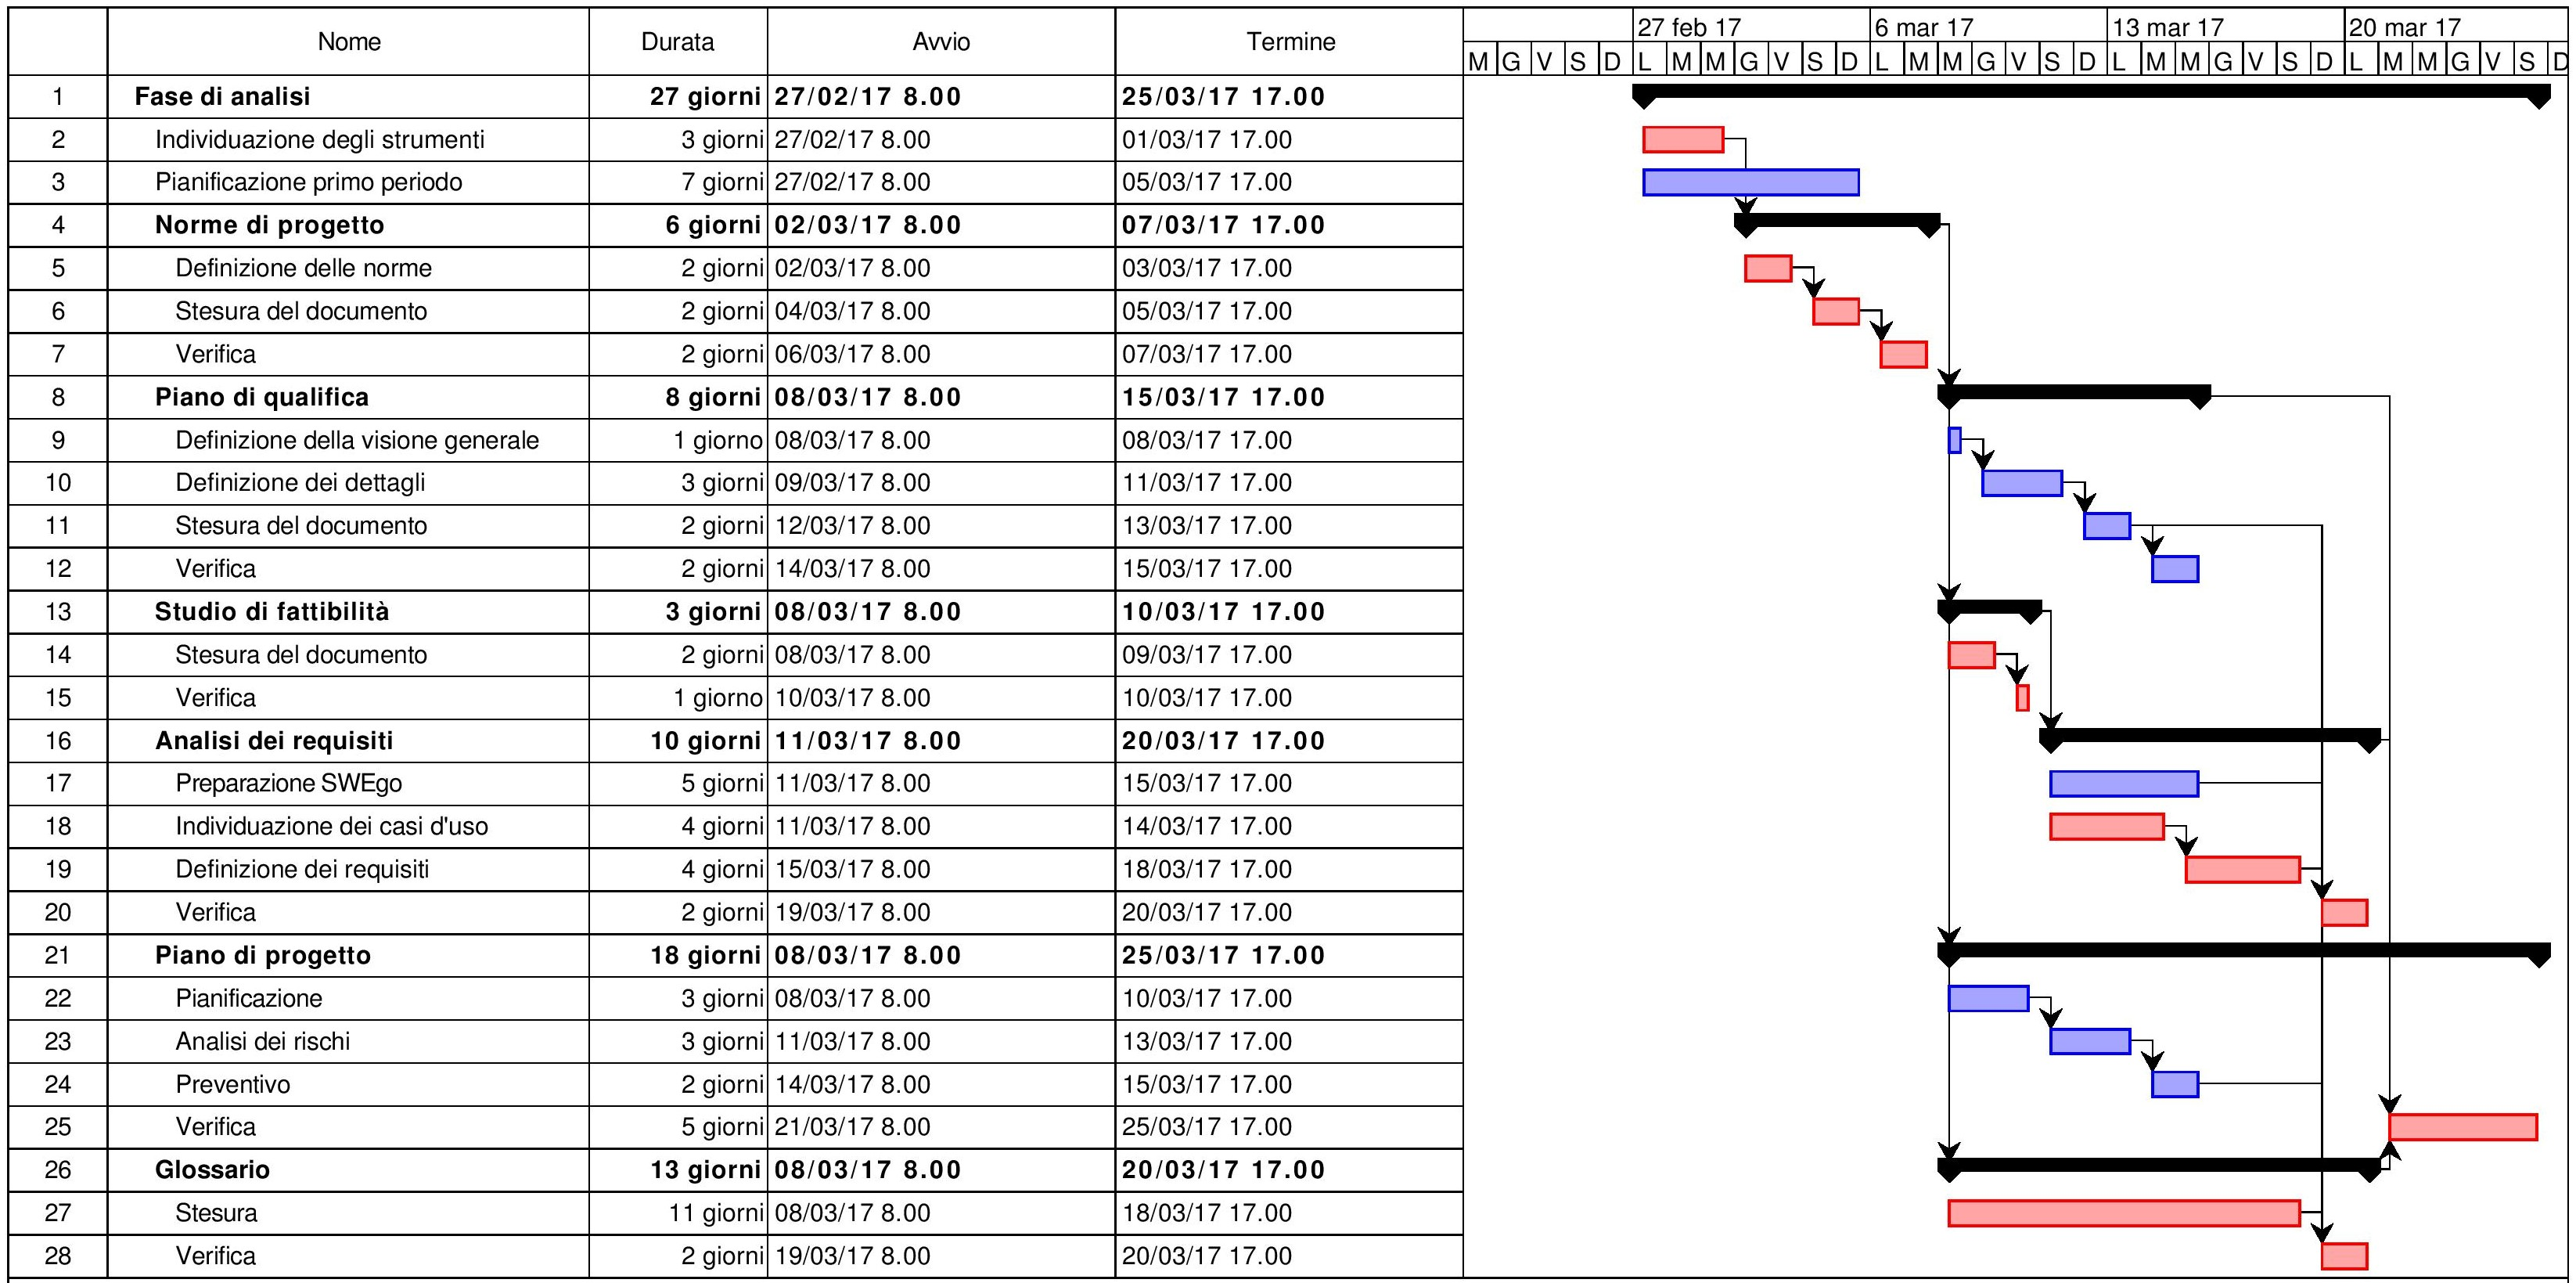
\includegraphics[scale=0.55]{Figures/Gantt_Analisi.jpg}
			\caption{Analisi: Diagramma di Gantt}
		\end{figure}
			
			
			
		\subsection{Analisi di dettaglio}
		\textbf{Periodo} : Da 26/03/2017 a 03/04/2017. \\
		Questo periodo comincia con la fine del periodo di analisi e prosegue fino alla scadenza della consegna della \revisionedeirequisiti.
		\begin{itemize}
			\item \textbf{Analisi di dettaglio}: si approfondisce quanto svolto in sede di analisi e si migliora in particolare il documento \analisideirequisiti;
			\item \textbf{Incremento e Verifica}: se necessario vengono aggiornati e verificati i documenti redatti in precedenza.
		\end{itemize}
		% DIAGRAMMA DI GANTT DELLE ATTIVITÀ
		\begin{figure}[H]
			\centering
			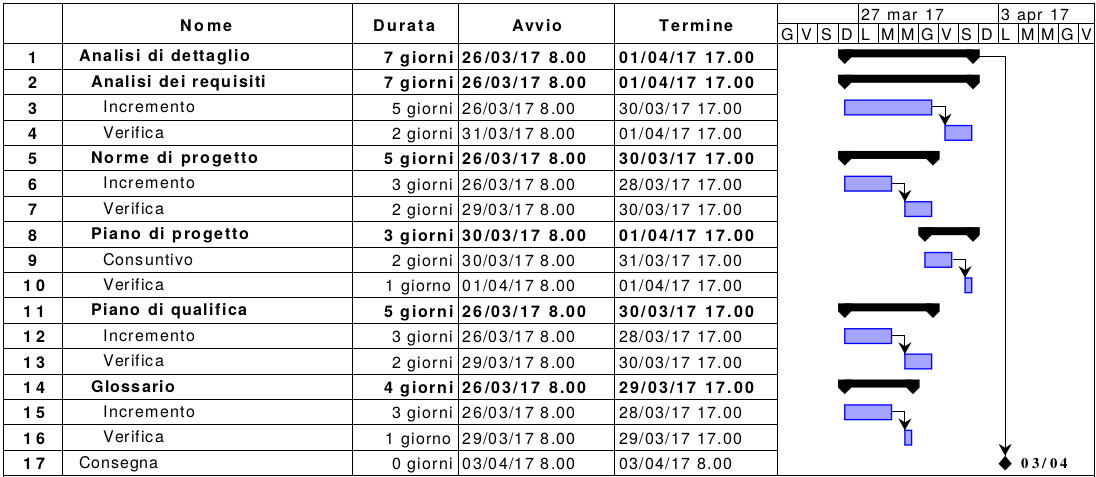
\includegraphics[scale=0.55]{Figures/Gantt_AnalisiDettaglio.jpg}
			\caption{Analisi di dettaglio: Diagramma di Gantt}
		\end{figure}
	
	
	
		\subsection{Progettazione architetturale}
		\textbf{Periodo} : Da 04/04/2017 a 27/04/2017. \\
		Questo periodo comincia al termine del periodo di Analisi di dettaglio e termina con un incontro di presentazione ufficiale con il proponente.
		\begin{itemize}
			\item \textbf{Specifica Tecnica}: dopo un primo periodo di auto formazione necessaria alla successiva progettazione ad alto livello del sistema viene redatta la \specificatecnica, dove sono esposte le scelte progettuali di alto livello del prodotto finale. Sono qui descritti i design pattern utilizzati, l'architettura generale del prodotto e il tracciamento dei requisiti;
			\item \textbf{Incremento e Verifica}: se necessario vengono aggiornati e verificati i documenti redatti in precedenza.
		\end{itemize}
		% DIAGRAMMA DI GANTT DELLE ATTIVITÀ
		\begin{figure}[H]
			\centering
			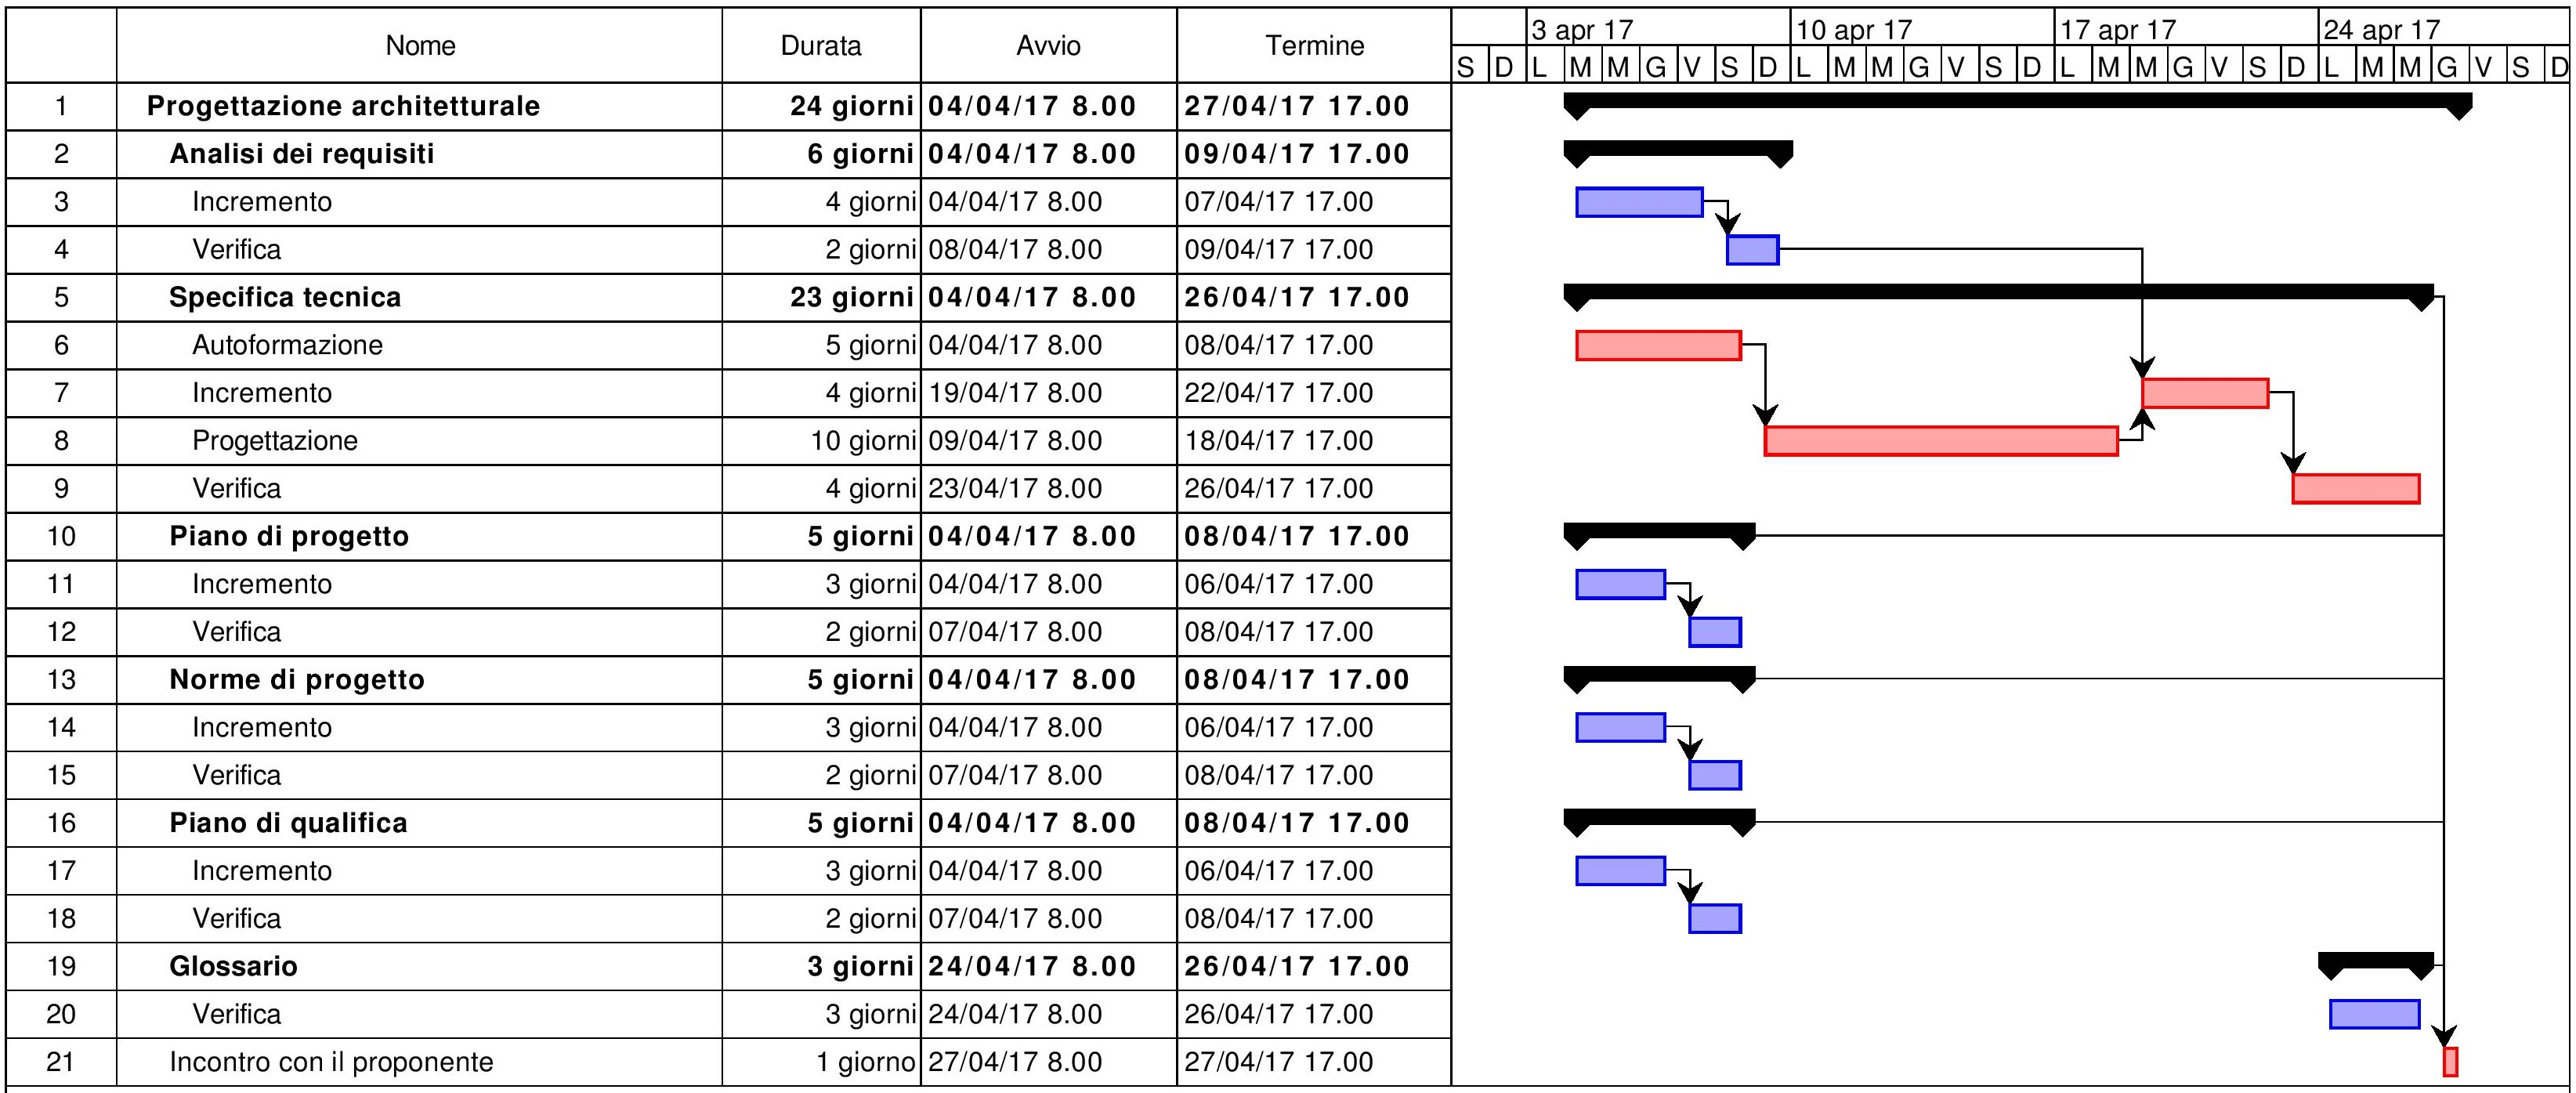
\includegraphics[scale=0.55]{Figures/Gantt_ProgettazioneArchitetturale}
			\caption{Progettazione architetturale: Diagramma di Gantt}
		\end{figure}
		
		
		
		\subsection{Progettazione di dettaglio e Codifica}
		\textbf{Periodo} : Da 28/04/2017 a 20/06/2017. \\
		Questo macro-periodo comincia al termine del periodo di Progettazione architetturale e prosegue fino alla scadenza della consegna della \revisionediqualifica.
		È a sua volta divisa in 3 grandi iterazioni che riguardano Progettazione di dettaglio e Codifica rispettivamente dei requisiti obbligatori, desiderabili e opzionali.
		\begin{itemize}
			\item \textbf{Definizione di prodotto}: si definiscono approfonditamente la struttura e le relazioni dei vari componenti del prodotto, in accordo con quanto descritto nella \specificatecnica. In base a questi viene redatta la \definizionediprodotto;
			\item \textbf{Codifica}: inizia in questo periodo lo sviluppo del codice del prodotto, seguendo la struttura stabilita dalla \definizionediprodotto;
			\item \textbf{Manuale Utente e Manuale Amministratore}: contestualmente alla progettazione di dettaglio del prodotto si redigono i manuali contenenti le linee guida per l'utilizzo del prodotto; 
			\item \textbf{Incremento e Verifica}: se necessario vengono aggiornati e verificati i documenti redatti in precedenza.
		\end{itemize}
		% DIAGRAMMA DI GANTT DELLE ATTIVITÀ
		\begin{figure}[H]
			\centering
			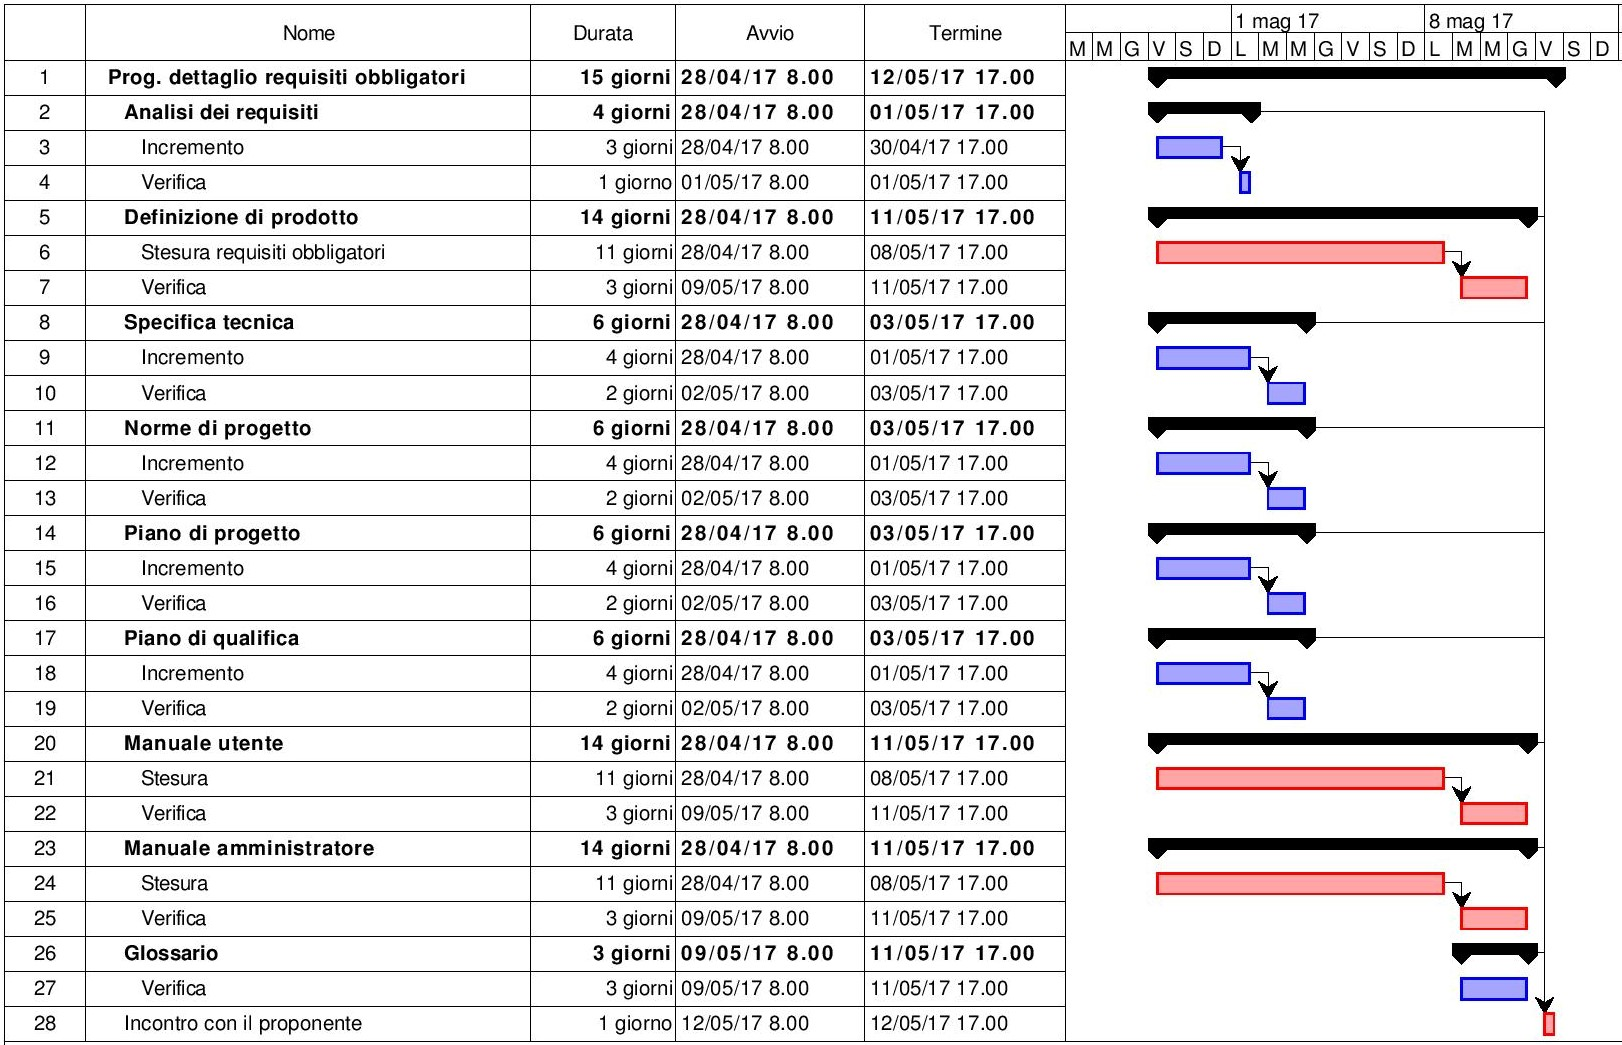
\includegraphics[scale=0.55]{Figures/Gantt_DettaglioObbligatori}
			\caption{Progettazione di dettaglio e Codifica: Diagramma di Gantt}
		\end{figure}
		\begin{figure}[H]
			\centering
			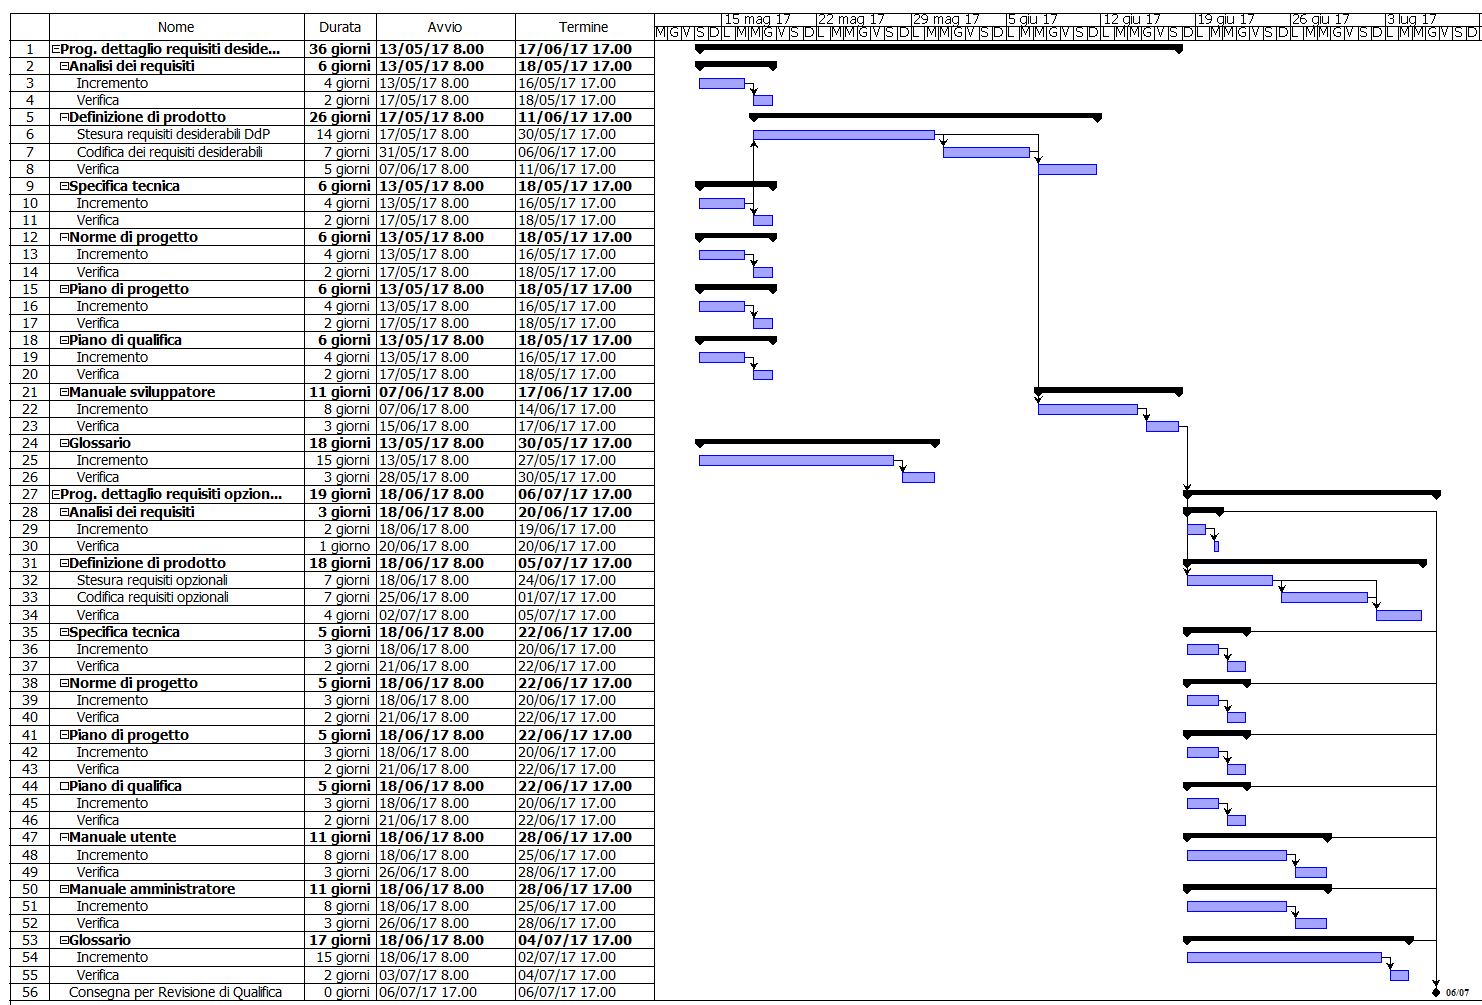
\includegraphics[scale=0.7]{Figures/Gantt_DettaglioOpz}
			\caption{Progettazione di dettaglio e Codifica: Diagramma di Gantt}
		\end{figure}
	
	
		
		\subsection{Validazione}
		\textbf{Periodo} : Da 21/06/2017 a 06/07/2017. \\
		Questo periodo comincia alla fine del periodo di Progettazione di dettaglio e Codifica e prosegue fino alla scadenza della consegna della \revisionediaccettazione.
		\begin{itemize}
			\item \textbf{Validazione}: si controlla che il prodotto soddisfi i requisiti specificati nel documento di \analisideirequisiti ;
			\item \textbf{Collaudo}: il prodotto viene testato in ogni funzionalità richiesta dal capitolato;
			\item \textbf{Incremento e Verifica}: se necessario vengono aggiornati e verificati i documenti redatti in precedenza;
			\item \textbf{Consegna}: il prodotto e i documenti prodotti vengono consegnati al committente durante la \revisionediaccettazione.
		\end{itemize}
		% DIAGRAMMA DI GANTT DELLE ATTIVITÀ
		\begin{figure}[H]
			\centering
			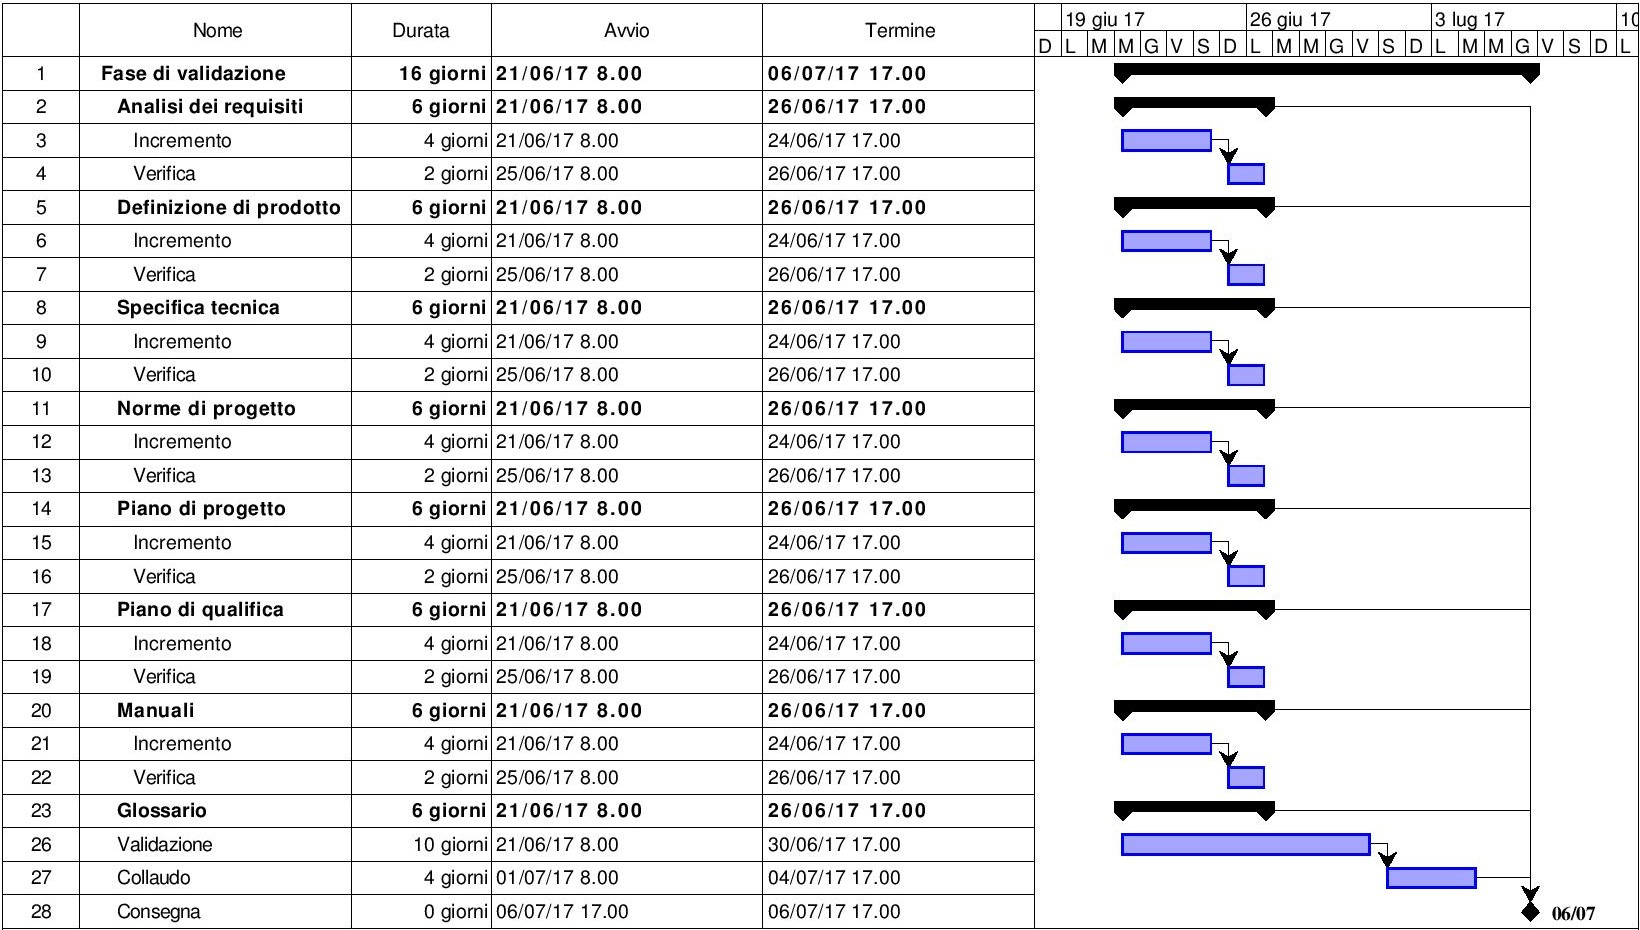
\includegraphics[scale=0.55]{Figures/Gantt_Validazione.jpg}
			\caption{Validazione: Diagramma di Gantt}
		\end{figure}
			
\end{document}
